
\documentclass[monografia]{tcc-abntex2}



% ---
% PACOTES
% ---
%\usepackage{cmap}				% Mapear caracteres especiais no PDF
\usepackage{pslatex}			% Usa a fonte Times News Roman			
\usepackage{makeidx}            % Cria o indice
\usepackage{hyperref}  			% Controla a formação do índice
\usepackage{lastpage}			% Usado pela Ficha catalográfica
\usepackage{indentfirst}		% Indenta o primeiro parágrafo de cada seção.
\usepackage{nomencl} 			% Lista de simbolos
\usepackage{graphicx}			% Inclusão de gráficos
\usepackage{lipsum}				% para geração de dummy text
\usepackage{float}
\usepackage[printonlyused]{acronym}
\usepackage{algpseudocode,algorithm}
%\usepackage[table]{xcolor}

%criar um novo estilo de cabeçalhos e rodapés
\makepagestyle{tccraiza}
  %cabeçalhos
  \makeevenhead{tccraiza} %pagina par
     {}
     {}
     {\thepage}
  \makeoddhead{tccraiza} %pagina ímpar ou com oneside
     {}
     {}
     {\thepage}
  \makeheadrule{tccraiza}{\textwidth}{\normalrulethickness}
  % rodapé
  %\makeevenfoot{tccraiza}
     %{rodapé par à esquerda} %pagina par
     %{centro \thepage}
     %{direita} 
  %\makeoddfoot{tccraiza} %pagina ímpar ou com oneside
    % {rodapé ímpar/onside à esquerda}
     %{centro \thepage}
     %{direita}


% ----------------------------------------------------------
\makeindex
% ----------------------------------------------------------
% Compila a lista de abreviaturas e siglas
% ----------------------------------------------------------
\makenomenclature
% ----------------------------------------------------------
% Inserir folha de aprovação digitalizada com as assinaturas
% ----------------------------------------------------------
%\inserirfolhaaprovacao{folhaAprovacao.pdf}


% ----------------------------------------------------------
% Início do documento
% ----------------------------------------------------------

\begin{document}



% ----------------------------------------------------------
% ELEMENTOS PRÉ-TEXTUAIS
% ----------------------------------------------------------
\pretextual
\pagenumbering{roman}
% Insere Capa, Folha de rosto e folha de aprovação (se inserida).
\thispagestyle{empty}
\begin{center}

------------------------------------------------------------------------------------------------------------
\normalsize{Curso de Ciência da Computação \\ Universidade Estadual de Mato Grosso do Sul}
------------------------------------------------------------------------------------------------------------

\vspace*{3cm}

\Large{ESTUDO E ANÁLISE DE MÉTODOS PARA RECONHECIMENTO DE PALAVRAS DITAS}


\vspace*{3cm}
\normalsize{Raiza Artemam de Oliveira \\ Willian Sousa Santos}

\vspace*{2cm}

\normalsize{Prof. MSc. André Chastel de Lima (Orientador)}

\vspace*{6cm}


\large{DOURADOS-MS \\ 2016}
\end{center}
\include{preTextual/contracapa}
\thispagestyle{empty}
\begin{center}

\Large{Estudo e Análise de Métodos para Reconhecimento de Palavras Ditas}

\vspace*{4cm}

\large{Raiza Artemam de Oliveira \\ Willian Sousa Santos }

\vspace*{4cm}

\end{center}
\begin{flushright}
\begin{minipage}{0.5\textwidth}
\normalsize{
Este exemplar corresponde à redação final
da monografia da disciplina Projeto Final de Curso 
devidamente corrigida e defendida por
 Raiza Artemam de Oliveira e Willian Sousa Santos
e aprovada pela Banca Examinadora, 
como parte dos requisitos para a obtenção
do título de Bacharel em Ciência da Computação.

\vspace*{2cm}

Dourados, xx de novembro de 2016

\vspace*{2cm}

Prof. MSc. André Chastel de Lima
}
\end{minipage}
\end{flushright}




\thispagestyle{plain}
\begin{center}

------------------------------------------------------------------------------------------------------------
\normalsize{Curso de Ciência da Computação \\ Universidade Estadual de Mato Grosso do Sul}
------------------------------------------------------------------------------------------------------------

\vspace*{2cm}

\LARGE{ESTUDO E ANÁLISE DE MÉTODOS PARA RECONHECIMENTO DE PALAVRAS DITAS}


\vspace*{1.5cm}
\normalsize{Raiza Artemam de Oliveira \\ Willian Sousa Santos}

\vspace*{1.5cm}

\normalsize{Outubro de 2016}

\vspace*{3cm}
\end{center}
\begin{flushleft}
\begin{minipage}{0.5\textwidth}
\normalsize{
BANCA EXAMINADORA:\\


Prof. MSc. André Chastel Lima (Orientador) \\
Área de Computação – UEMS\\



Profa. [Titulação]  Nome do professor \\
 Área de Computação – UEMS\\


 Profa. [Titulação] Nome do professor \\
 Área de Computação – UEMS 
}
\end{minipage}
\end{flushleft}



% Pequena dedicatpertinente ao seu 
% trabalho ou que represente o seu modo de pensar.) 
% 
%
% Arquivo: dedicatoria.tex
% ----------------------------------------------------------------------- %
\thispagestyle{plain}
\vspace*{\fill}

{ \raggedleft


\textit{Computer science is no more about computers than astronomy is about telescopes, biology is about microscopes or chemistry is about beakers and test tubes. Science is not about tools, it is about how we use them and what we find  out when we do.. \\
Edgar Dijkstra}

~
}
% ----------------------------------------------------------------------- %
% Um pequeno texto para agradecer m de maneira
% relevante o do trabalho 
%
% Arquivo: agradecimentos.tex
% ----------------------------------------------------------------------- %

\chapter*{Agradecimentos}
\thispagestyle{plain}
\normalsize{thanks  ;*


}.

% ---
%\maketitle

\begin{resumo}{Áudio, HMM, SOM }
\label{sec:resumo}
\quad Esta dissertação irá tratar de alguns algoritmos para reconhecimento de fala, mas para isso, realizamos todo o processo de captação, tratamento do áudio, junto com a implementação dos algoritmos(HMM e SOM). É utilizado um transdutor para a captação do áudio, transformando  ondas analógicas em ondas digitais, utilizamos o ALSA, que oferece algumas interfaces, a que principalmente utilizamos, foi a interface de tempo e de captaç/ão de audio, após essa captura realizamos o que chamamos de pré-enfase, que consiste em retirar, ou pelo menos diminuir aquilo que não precisamos, (ruidos, ecos, etc) ou qualquer tipo de interferência, e maximizar as informações úteis (voz do interlocutor), após a realização da pré-enfase, implementou-se em linguagem c, os algoritmos HMM e SOM, para avaliarmos que dado um vocabulário finito pré-armazendo, e apontar a melhor solução para reconhecimento de palavras ditas em ambientes não controlados.\\


\end{resumo}
\sumario
\listasiglas{abrev/Abreviaturas}
\listatabelas
\listafiguras


% ----------------------------------------------------------
% ELEMENTOS TEXTUAIS
% ----------------------------------------------------------
\pagenumbering{arabic} % volta à numeração arábica
\pagestyle{tccraiza}
% ----------------------------------------------------------
% Introdução, Desenvolvimento e Conclusão
% ----------------------------------------------------------
\chapter{INTRODUÇÃO}
\label{chap:introducao}
 \thispagestyle{plain}


\quad Nos primeiros sistemas computacionais a comunicação entre pessoas e máquinas era realizada através de terminais por linha de comando.  Apenas especialistas conseguiam utilizar estes sistemas.
Depois, no início da década de 70, com a criação do mouse e a introdução da interface gráfica  os sistemas tornaram-se mais amigáveis ao usuário, podendo ser utilizados por pessoas comuns sem necessidade de conhecimento técnico. Com o passar dos anos a interação entre pessoas e máquinas tornou-se mais intuitiva com as diversas interfaces entre o usuário e o sistema. No fim da década de 70 iniciaram-se as pesquisas de reconhecimento de fala.
Interfaces por meio de fala são utilizadas em diversas áreas, tais como: sistemas embarcados, automação residencial, operações bancárias, conversão fala texto e dispositivos móveis.

\quad O reconhecimento da fala é um campo de estudo amplo e necessário as diversas tecnologias que utilizam
desta como um  meio de comunicação entre o usuário e o sistema. Utilizar a fala como entrada de um sistema
torna a comunicação entre o usuário e o sitema mais direta, intuitiva, rápida e precisa.Como um campo de ampla aplicacação, o reconhecimento de fala tem diversos projetos em diferentes partes do mundo. Dentre os quais se destaca o projeto CMU Sphinx da universidade americana Carnegie Mellon. O projeto já tem cerca de 20 anos de pesquisas na área de reconhecimento de fala e de voz. Trata-se de um projeto open source voltado para linux, mas também conta com uma versão em java multiplataforma. O CMU Sphinx oferece suporte para várias linguagens, dentre elas o inglês, alemão, russo, francês e espanhol. 
O reconhecimento de fala pode ser classificado de acordo com o tamanho do vocábulario, de acordo com os algoritmos utilizados e de acordo com o tipo de fala a ser reconhecida (contínua ou discreta).



%A introdução deve conter a delimitação do tema, o problema, a justificativa e o
%objetivo do projeto, que podem vir em subseções separadas ou não.
%É muito importante ressaltar que a delimitação do tema requer clareza a respeito do
%campo de conhecimento a que pertence o assunto. O problema é o objeto de pesquisa ou de
%estudo. Optou-se, neste exemplo, em separar em subseções a justificativa e o(s) objetivo(s).\\
%No caso de projeto de pesquisa, que esteja vinculado a um grupo de pesquisa
%institucional, neste item é necessário acrescentar a denominação do grupo, que esteja
%devidamente certificado pela Unifra, e a denominação da linha de pesquisa a que pertence o
%projeto

\section{Justificativa}
\label{sec:justificativa}



O reconhecimento de palavaras ditas é um campo de estudo de extrema importância para uma melhor comunicação entre usuários e sistema.
%Na justificativa mencionam-se a relevância científica do trabalho, a contribuição da
%pesquisa e que benefício poderá trazer à comunidade ou à sociedade. Ainda devem estar claros
%o motivo da escolha do tema e as possibilidades de realização da pesquisa.
\section{Objetivos}
\label{sec:objetivos}

O objetivo deste trabalho é estudar os principais métodos de reconhecimento de fala. Analisar os algoritmos utilizados, suas vantagens e desvantagens. Apresentar os resultados para um pequeno vocábulario.
%A definição dos objetivos determina o que se quer atingir com a realização do
%trabalho de pesquisa. Objetivo é sinônimo de meta, fim.
%Uma sugestão interessante, na redação dos objetivos, é utilizar, no início das
%sentenças, o verbo no infinitivo, tais como: esclarecer tal coisa, definir tal assunto, procurar
%aquilo, permitir algo, demonstrar alguma coisa, entre outros.
%Alguns autores separam os objetivos em objetivo geral e objetivos específicos, mas
%não há regra a ser cumprida quanto a isso. Caso se opte em separá-los, tem-se:
\subsection{Objetivo geral}
\label{subsec:objetivogeral}
Estudar e analisar os algoritmos existentes para o reconhecimento de palavras  ditas em um vocábulario pequeno e um ambiente não controlado.
%O objetivo geral vincula-se à própria significação geral do tema proposto pelo
%projeto, ou seja, significa traçar as principais metas que norteiam a pesquisa.
\subsection{Objetivo específico}
\label{subsec:objetivoespecifico}
%Descrever aqui o(s) propósito(s) específico(s) para atingir um ponto de vista do tema,
%um ângulo a ser pesquisado, permitindo atingir o objetivo geral. Aconselha-se, na redação
%desta seção, não ser prolixo.
Apontar a melhor solução para reconhecimento de palavras ditas em ambientes não controlados.


\section{Metodologia}

\quad A metodologia adotada para a realização deste trabalho consiste nos seguintes passos:

\begin{itemize}
\item Pesquisa em livros, sites, artigos e notas de aula sobre o tema abordado e seus diversos aspectos;
\item Estudo de algoritmos aplicados ao reconhecimento de fala;
\item Implementação computacional de algoritmos aplicados ao reconhecimento de fala;
\item Testes e validação dos algoritmos implementados;
\item Análise e validação dos resultados obtidos com os métodos implementados;
\item Documentação do trabalho. 

\end{itemize}

\quad No capítulo \ref{chap:referencial_teorico} é feita uma explicação do que é relevante para este trabalho com base na literatura.


























\chapter{FUNDAMENTAÇÃO TEÓRICA}
\label{chap:referencial_teorico}
\thispagestyle{plain}
De acordo com \cite{fundRecFala}, os  sistemas de reconhecimento de fala podem ser classificados em três grupos de acordo com a técnica utilizada. Estes grupos são :
\begin{itemize}
\item Reconhecedores por inteligência artificial;
\item Reconhecedores por comparação de padrões;
\item Reconhecedores baseados na análise acústico-fonética.
\end{itemize}
\section{Sistemas de reconhecimento de fala }

\label{sec:sistemasdereconhecimentodefala}


\subsection{Reconhecedores baseados em inteligência artificial}

Os sistemas de reconhecimento de fala que utilizam a inteligência artificial usa propriedades tanto dos reconhecedores por comparação de padrões quanto dos reconhecedores baseados na análise acústico-fonética. Sistemas com redes neurais são encaixados nesta classe. As redes Multilayer Perceptron usam uma matriz de ponderação que representa as conexões entre os nós da rede, e cada saída esta associada a uma unidade a ser reconhecida \cite{kluwerNeural}.

A abordagem de inteligência artificial se baseia no processo humano natural de ouvir, analisar e tomar uma decisão sobre as características acústicas medidas para reconher a fala. Faz parte do processo de reconheciemento de fala pela abordagem de inteligência artificial o processo de segmentação e rotulagem usado na análise acústico-fonética  \cite{fundRecFala}. Esta abordagem aplica o conceito de que o conhecimento é dinâmico  e os modelos devem adaptar-se frequentemente. 

\subsection{Reconhecedores por comparação de padrões}

Estes reconhecedores usam o príncipio de que o sistema foi treinado para reconhecer os padrões. Os sistemas por reconhecimento de padrões possuem duas fases diferentes :
\begin{itemize}
\item Treinamento;
\item Reconhecimento.
\end{itemize}

Durante a fase de treinamneto são criados padrões de referência para o sitema. Na fase de reconhecimento compara-se os padrões obtidos com os padrões de referência criados na fase anterior e calcula-se uma medida de similaridade entre os padões. O padrão mais similar ao desconheido é escolhido como reconhecido. Os sistemas que se baseiam nos Modelos Ocultos de Markov (HMM) se encaixam nesta categoria.\\

Dentre as diversas razões para usar a abordagem de comparação de padrões para reconheimento de fala podemos citar a simplicidade de uso, por ser um método de fácil entendimento que possui uma rica fundamentação matemática e é amplamente utilizado,  e a robustez, trata-se de um método robusto e invariante para diferentes vocábularios, algoritmos de comparação de padrão e regras de decisão. Isto torna esta abordagem apropriada para uma vasta gama de unidades de fala, como fonemas, palavras isoladas ou frases  \cite{fundRecFala}. 

\subsection{Reconhecedores baseados na análise acústico-fonética}

Os sistemas baseados na análise acústico-fonética decodificam o sinal de fala  baseados nas características acústicas deste sinal e na relação entre elas \cite{kluwer}. Os sistemas de análise desta classe devem considerar propriedades acústicas invariantes. Entre estas características estão a classificação entre sonoro e não sonoro, segmentção do sinal da fala, detecção das características que descrevem as unidades fonéticas e escolha do padrão que mais corresponde à sequencia de unidades fonéticas.\\

Os reconhecedores baseados na análise acústico-fonética trabalham em duas etapas. O primeiro passo na análise acústico fonética é chamado de fase de segmentação e rotulagem \cite{fundRecFala}. Este passo envolve a segmentação do sinal da fala em regiões discretas, no tempo, onde as propriedades acústicas do sinal são representadas por um único fonema, ou estado. Em seguida uma ou mais etiqueta fonética é associada a cada região segmentada de acordo com as propriedades acústicas. O segundo passo para o reconhecimento tenta determinar uma palavra válida a partir da sequência de etiquetas fonéticas obtidas na fase anterior. As palavras são obtidas a partir de um determinado vocabulário, as palavras obtidas fazem sentido sintático e tem significado semântico.

\section{Processamento digital de sinais}
 
De acordo com \cite{sig} um sinal é qualquer função associada a um fenômeno físico, econômico ou social e que transporta  algum tipo de informação sobre ele. Pode ser definido como uma descrição quantitativa de um dado fenômeno. A voz é um exemplo de sinal.\\ Os sinais podem ser classificados de diferentes formas de acordo com suas características  e com o tipo de domínio e contradomínio. Segundo \cite{sig} esta classificação pode ser feita de acordo com as seguintes características:
\begin{enumerate}
\item Variável independente: o sinal é contínuo se $t \in \mathbb{R}$ e discreto se $t \in \mathbb{Q}$. Os pontos $t_n, n \in \mathbb{Z}$ são chamados de instantes de amostragem. Sinal amostrado é o sinal discreto obtido por amostragem de um sinal contínuo.

\item Amplitude: os sinais podem ser classificados de acordo com a amplitude em :
\begin{itemize}
\item Analógicos: sinal contínuo cuja amplitude pode assumir uma gama contínua de valores;
\item Quantificados: sinal cuja amplitude pode assumir, apenas, uma gama finita de valores;
\item Digitais: sinal resultante da codificação de um sinal amostrado e quantificado. A codificação consiste em atribuir a cada valor obtido por amostragem e quantificação  um código.
\end{itemize} 
\item Duração: os sinais cujo dominio é limitado dizem-se de duração finita, os restantes são de duração infnita.Os sinais de duração finita tambem são chamdos de janela.
\item Reprodutibilade: um sinal é dito determinístico se repetindo a mesma experiência obtém-se o mesmo resultado, caso isso não seja possível  então trata-se de um sinal aleatório.
\item Periodicidade: os sinais determinísticos classificam-se ainda em aperiódicos e periódicos. Os sinais aperiódicos nao são repetitivos. Os sinais periódicos são repetitivos e possuem a relação $x(t) = x(t \bar{+} T) \quad \forall \quad t$, onde $T$ é o período. Quando $T < 2 \pi$ a involvente final do sinal periódico $x(t)$ não coincide com a extensão periódica do sinal base $x_b(t)$ ocorre o fenômeno chamado \textit{aliasing}. O fenômeno de aliasing é importante na conversão discreto-contínua e verifica-se no domínio da frequência.
\item Morfologia: formas simétricas a um eixo ou outro. Os sinais pares são simétricos ao eixo das ordenadas. Os sinais impares são simétricos ao eixo das abscissas.
\item Carater : outras medidas são consideradas. Um sinal pode ter carater escalar, vetorial. Por exemplo o sinal de saída de uma gregado de sensores é um sinal sensorial.
\end{enumerate}

A análise frequencial moderna é um conjunto de técnicas matemáticas e ou físicas que permite  obter o conteúdo frequêncial de qualquer sinal , a que se chama de espectro. O processo de obtenção de espectro chama-se análise espectral. O processo numérico usado para determinar o espectro é chamado de estimação espectral. A estimação espectral é feita em sinais de fonte fisica, como a voz, durante um intervalo de tempo finito. Na prática o conteúdo frequêncial de um dado sinal não é uniforme. Assume valores significativos em intervalos chamados bandas. A designação de filtro habitualmente usada em referência aos sistemas lineares, deriva da possibilidade de certos sistemas eliminarem ou atenuarem fortemente certas bandas. A Tabela \ref{tab:banda}
mostra alguns sinais e suas bandas.

\begin{table}[H]
\centering
\caption{Bandas ocupadas por alguns sinais}
\label{tab:banda}
\smallskip
\begin{tabular}{|l|l|l|}
\hline
Sinal  & de & a\\[0.5ex]
\hline
&&\\[-2ex]
Eletrocardiograma& 0 Hz & 150 Hz \\[0.5ex]
\hline
&&\\[-2ex]
Eletroencefalograma& 0 Hz & 100 Hz\\[0.5ex]
\hline
&&\\[-2ex]
Voz & 100 Hz & 4000 Hz\\[0.5ex]
\hline
&&\\[-2ex]
Ruído do vento& 100 Hz &1000 Hz \\[0.5ex]
\hline
&&\\[-2ex]
Ruído de tremor de terra& 0.01 Hz& 10 Hz \\[0.5ex]
\hline
&&\\[-2ex]
Radiodifusão& 0.03 MHz& 3 MHz\\[0.5ex]
\hline
&&\\[-2ex]
Onda curta& 3 GHz & 30 GHz\\[0.5ex]
\hline
&&\\[-2ex]
Radar, satélite, comun. espaciais& 300 GHz & 300 THz \\[0.5ex]
\hline
&&\\[-2ex]
Luz visível& 370 THz& 770 THz \\[0.5ex]
\hline
\end{tabular}
\end{table}






























%alguns exemplos de citação:\\
%\cite{berquo1980fatores}\\
%\cite{santos1980dinamica}\\
%\cite{NBR6023:2002}\\
%\cite{NBR14724:2005}\\
%\cite{NBR10520:2002}\\
%\cite{lessa2004manual}\\
%\cite{rey2000planejar}\\
%\cite{rajagopalan2003identidade}\\
%\cite{flemming1999calculo}\\
%\cite{gonccalves2}\\
%\cite{salgado2002nutriccao}
\chapter{CAPTURA DE ÁUDIO}
\label{chap:cap_audio}
\thispagestyle{plain}
\quad A captura do sinal de áudio é uma parte fundamental para o desenvolvimento de um sistema reconhecedor de fala. Existem bases de dados disponíveis para testes em que a captura
do sinal de áudio não é necessária, um vez que estas bases disponibilizam os arquivos de áudio. Um exemplo de base de dados de voz é a Aurora-1, esta base é construída por sinais de fala   limpos e degradados através de oito tipos de ruídos \cite{aurora}. Neste trabalho optamos por realizar a captura do áudio pois este também faz parte do objetivo.\\ 
O som se propaga no ambiente por meio de ondas de forma contínua no tempo e no espaço a uma velocidade média de \textit{340 metros/segundo} fazendo o ar vibrar. Esta onda sonora  é capturada por meio de um microfone como uma onda analógia e  é convertida para um sinal digital. A onda capturada é normalizada através de um filtro de passa-baixas. Circuitos que realizam esta conversão de onda são chamados de  ADC (\textit{ analog digital converter}). O tamanho das amostras, expressa em bits, é um dos fatores que determina a precisão com que o som é representado em forma digital. Outro fator importante que afeta a qualidade de som é a taxa de amostragem. O teorema de Nyquist  afirma que a frequência mais elevada que pode ser representado com precisão é, no máximo, metade da taxa de amostragem \cite{nyqui}.

\section{Bibliotecas para Captura de Áudio}
\quad Para o processo de reconhecimento de fala de qualquer tipo, primeiro é necessário capturar o sinal de áudio. A fase de captura de áudio é essencial para o bom desempenho do projeto. Existem diversas bibliotecas open-source que oferecem funções que realizam a captura e gravação de áudio, entre elas a Allegro e OpenGL, entretanto a aplicação dessas bibliotecas implica em um maior custo computacional, uma vez que estas trazem milhares de linhas de código junto com outras funções além das necessárias para a implementação deste projeto. Com base nisso, buscou-se uma alternativa que integrasse eficiência e baixo custo computacional para aplicações em áudio. 
 
\subsection{ALSA}
\quad ALSA (\textit{advanced linux sound architeture }) consiste de um conjunto de drivers do kernel, uma biblioteca, uma API e programas utilitários para o suporte de som no linux. Jaroslav Kysela iniciou o projeto ALSA porque os drives de som do kernel Linux não estavam sendo devidamente mantidos e atualizados. Após  a iniciativa mais desenvolvedores aderiram ao projeto e a estrutura da API foi refinada. ALSA foi incorporada ao kernel oficial do Linux 2.5.
A biblioteca fornecida pelo ALSA, libasound, fornece uma nomeação lógica dos dispositivos de hardware. Os nomes podem ser de dispositivos de hardware reais ou plugins \cite{linux}. Os dispositivos de hardware usam o formato $HW:i,j$, onde $i$ é o número do cartão e $j$ do dispositivo do cartão. Uma placa de som tem um buffer de hardware que armazena amostras gravadas. Quando este buffer enche, ele gera uma interrupção. O driver de som do kernel, em seguida, utiliza o acesso direto à memória  para transferir as amostras para um buffer de aplicativo na memória. O tamanho deste buffer pode ser  programado por chamadas da biblioteca ALSA. Caso o buffer seja muito grande a tranferencia geraria uma latência excessiva. ALSA resolve isso dividindo o buffer em fragmentos e transfere os dados fragmentados. A Figura \ref{fig:pcm} ilustra a repartição do buffer em fragmentos, molduras e amostras.

\begin{figure}[H]
\centering % para centralizarmos a figura
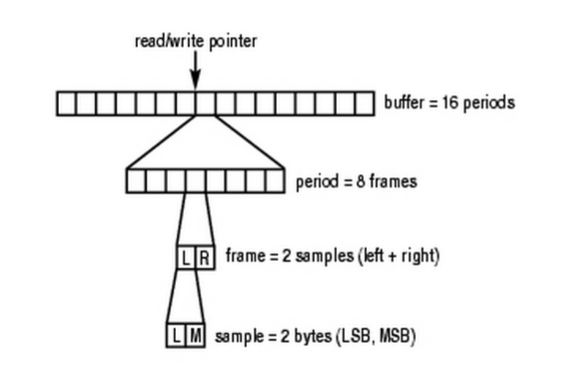
\includegraphics[width=10cm]{img/pcm.jpg} % leia abaixo
\caption{Buffer de aplicação. \textit{fonte:\cite{linux}}}
\label{fig:pcm}
\end{figure}

\quad A API ALSA oferece seis principais interfaces. São elas  a interface de controle, interface MIDI raw, interface de tempo, interface de sequência, interface mixer e interface de PCM. Esta última gerencia a captura e reprodução de áudio digital. 


\section{Arquivos WAVE}

\quad O formato de áudio adotado foi o WAVE. Neste tipo de formato o som é armazenado em sequências numéricas. O áudio é convertido em dados e armazenado bit a bit. O WAVE (.wav) foi criado pela IBM e pela Microsoft, nos anos oitenta e tem suporte a  uma série de resoluções de bit, taxas de amostragens e canais de áudio.  A taxa de amostragem em arquivo .wav refere-se ao número de amostras por segundo. O CD possui uma taxa de amsotragem de $44,100$, o que significa que cada segundo de áudio tem $44,100$ amostras. A quantidade de bits usada determina  quanta informação pode ser armazenada  no arquivo. A quantidade de bits também interfere na amplitude do sinal. Em uma gravação de 8 bits estará disponível 256 níveis de amplitude, variando de $0$ à $255$. Em uma gravação de 16 bits a quantidade de níveis de amplitude disponíveis passa a $65,536$, variando entre $-32,768$  até $32767$. A quantidade de 16 bits é suficiente para este projeto. 

\subsection{Cabeçalho WAVE}

\quad O cabeçalho de um arquivo .wav possui 44 bytes e é organizado como mostrado na Tabela \ref{tab:app}.

\begin{table}[H]
\centering
\caption{Formato de um cabeçalho de arquivo wave}
\label{tab:app}
\smallskip
\begin{tabular}{|l|l|l|}
\hline
Posição & Valor & Descrição\\[0.5ex]
\hline
&&\\[-2ex]
1 - 4& RIFF & Define como um arquivo RIFF \\[0.5ex]
\hline
&&\\[-2ex]
5 - 8& Tamanho do arquivo (int) & Tamanho máximo do arquivos em bytes \\[0.5ex]
\hline
&&\\[-2ex]
9 - 12 & "WAVE" & Arquivo tipo cabeçalho wave\\[0.5ex]
\hline
&&\\[-2ex]
13 - 16& "fmt" & Marca formato chunk \\[0.5ex]
\hline
&&\\[-2ex]
17 - 20& 16& Tamanho do formato dos dados \\[0.5ex]
\hline
&&\\[-2ex]
21 - 22& 1& Formato tipo PCM\\[0.5ex]
\hline
&&\\[-2ex]
23 - 24& 2 & Quantidade de canais\\[0.5ex]
\hline
&&\\[-2ex]
25 - 28& 44100 & Taxa de amostragem \\[0.5ex]
\hline
&&\\[-2ex]
29 - 32& 176400& (taxa de amostragem * bits por amostra * canais) / 8 \\[0.5ex]
\hline
&&\\[-2ex]
33 - 34&  4 & limites \\[0.5ex]
\hline
&&\\[-2ex]
35 - 36& 16 & Quantidade de bits por amostra \\[0.5ex]
\hline
&&\\[-2ex]
37 - 40& data & Marca o início da seção de dados \\[0.5ex]
\hline
&&\\[-2ex]
41 - 44& Tamanho do arquivo (dados) & Tamanho da seção de dados \\[0.5ex]
\hline
\end{tabular}
\end{table}




\chapter{PRÉ-PROCESSAMENTO}
 \thispagestyle{plain}
\label{chap:pre_proc}
Neste capítulo discutimos as técnicas usadas para o pré-processamento do sinal de áudio.
\quad O processo para reconhecimento de fala pode ser divido em várias etapas. O sinal de áudio é recebido do meio externo através de um transdutor e convertido para um sinal digital,
a partir deste momento devemos tratar este sinal. A  Figura \ref{fig:diaMFCC} ilustra as etapas do processo de extração de características \textit{mel-cepstrais}, também chamadas características \textbf{MFCC} (mel frequency cepstral coefficients).

\begin{figure}[H]
\centering % para centralizarmos a figura
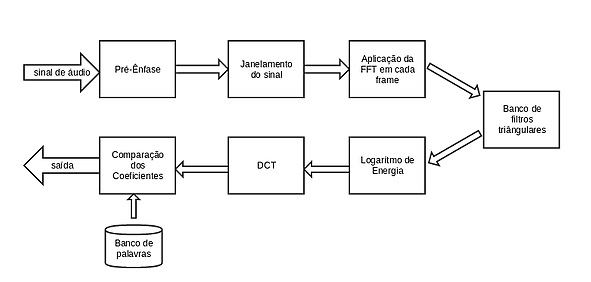
\includegraphics[width=10cm]{img/diaMFCC.jpg} % leia abaixo
\caption{Etapas para extração de coeficientes MFCC.}
\label{fig:diaMFCC}
\end{figure}

O sinal recebido deve passar pelo pré-processamento para reduzir as interferências externas do sinal e ressaltar as informações úteis. Durante a etapa de pré-ênfase o sinal é normalizado. A normalização da amplitude do sinal garante que sons em diferentes alturas sejam processados igualmente. Os períodos de silêncio do sinal são retirados para que apenas dados importantes sejam armazenados.\\ Após a etapa de pré-ênfase é realizado o janelamento do sinal, ou seja, o sinal é dividido em frames. É aplicada uma janela de Hamming para atenuar as descontinuidades causadas no início e final de cada frame.  A próxima etapa é a aplicação da Transformada Rápida de Fourier (FFT - do inglês \textit{fast fourier transform}) no sinal. A equação \ref{eqima} para obter a potência espectral.
\begin{equation}
\label{eqima}
S[k] = |X[k]|^2 = (real(X[k]))^2 +  (imaginaria(X[k]))^2
\end{equation}
 A FFT transforma um sinal do domínio do tempo para um do domínio da frequência.  A  Transformada Discreta de Fourier (DFT - do inglês \textit{discret fourier transform}) possui complexidade $O(n^2)$ e a FFT possui complexidade $O(n log n)$, por este motivo a FFT é usada em aplicações computacionais. A próxima etapa é a aplicação do banco de filtros triângulares, estes exigem uma explicação mais detalhada de como foram feitos. Esta explicação é feita em detalhes na seção \ref{sec:filt_tri}.

\section{Filtros Digitais}
\label{sec:filt:tri}
\quad Filtros digitais são usados para separar os sinais.  Para o processamento de áudio são aplicados os filtros no domínio da frequência, estes filtros selecionam certas regiões  no espectro, bloqueando as demais \cite{sig}. Aplicar diferentes filtros para o sinal de voz implica em diferentes técnicas. Em \cite{mello} e em \cite{pucpncc} é possível encontrar uma descrição mais detalhada para descritores de voz. Neste trabalho foi utilizado os filtros triângulares que estão diretamente realcionados a escala \textit{mel}, esta é explicada na seção seguinte. 

\subsection{Escala Mel}
\label{sec:mel}
\quad Em 1937 Stanley Smithy Stevens, John Volkman e Edwin Newmann propuseram o uso de uma variável psicoacústica chamada  \textbf {pitch}  para a criação de uma escala musical perceptual de tons em intervalos igualmente espaçados, chamada escala  \textbf {mel}. A frequência ouvida pelo sistema auditivo humano é subjetiva e varia de acordo com cada indivíduo. Esta impressão subjetiva de frequência é a sensação subjetiva da intensidade ou a amplitude de um som. A escala \textit{mel} é uma escala de pitches julgados pelos ouvintes como sendo igual em distância um do outro. O ponto de referência entre esta escala e a medição de freqüência normal é definida  igualando um tom de 1000 Hz , 40 dB acima do limiar do ouvinte , com um pitch de 1000 \textit{mels}. Abaixo de cerca de 500 Hz as escalas de \textit{mel} e Hertz coincidem, acima disso intervalos cada vez maiores são julgados por ouvintes para produzir iteração igual aos pitches. A escala \textit{mel} é baseada em um mapeamento entre a frequência real e o pitch aparentemente percebido do sistema auditivo humano. Para converter uma frequência em escala \textit{mel} aplica-se a equação \ref{melscale}, onde $f$ é frequência.
\begin{equation}
\label{melscale}
M(f) = 1125 ln(1 + \frac{f}{700})
\end{equation}

\subsection{Filtros Triângulares}
\label{sec:filt_tri}
A percepção humana de algumas frequências de sons complexos não podem ser individualmente dentro de certas bandas, quando uma dessas componentes cai fora da banda, chamada de banda crítica, ela pode ser identificada. Isto ocorre porque a percepção de uma frequência particular pelo sistema auditivo, por exemplo $f_0$, é influenciada pela energia da banda crítica das frequências em torno de $f_0$. O valor dessa banda varia nominalmente de $10 \%$ a $20 \%$ da frequência central do som, começando em torno de $100 Hz$ para frequências abaixo de $1 kHz$ e aumentando em escala logarítmica acima disso. Com base nestes fenômenos utiliza-se o logarítmo da energia total das bandas críticas em torno das frequências mel. A aproximação utilizada para este cálculo é a utilização de um banco de filtros espaçados uniformemente na escala mel, o banco de filtros triangulares. Os filtros \textit{mel} são definidos de acordo com a função \ref{filtro}.
\begin{equation}
\label{filtro}
%\begin{displaymath}
H_m[k] = \left\{\begin{array}{ll}
0 & k < k[m-1]\\
\displaystyle \frac{2(k-k[m-1])}{(k[m+1]-k[m-1])(k[m]-k[m-1])}, & k[m-1] \leq k \leq k[m] \\
\displaystyle \frac{2(k[m+1]-k)}{(k[m+1]-k[m-1])(k[m+1]-k[m])}, & k[m] \leq k \leq k[m+1] \\
0 & k > k[m+1]\end{array} \right.
%\end{displaymath}
\end{equation}
 Onde:
$M$ = números de filtros, $m$ = número do filtro, tal que $1 \leq m \leq M$ e $f(m)$ = frequência central de cada filtro.\\

A Figura \ref{fig:filtro} mostra o banco de filtros usados na técnica MFCC. Cada filtro calcula a média do espectro em torno de um espectro central. Quanto maior a frequência, maior é a largura da banda.

\begin{figure}[H]
\centering % para centralizarmos a figura
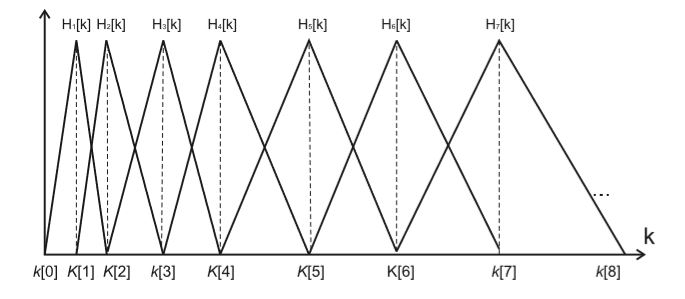
\includegraphics[width=10cm]{img/filtrotriangular.jpg} % leia abaixo
\caption{Banco de filtros triângulares MFCC. \textit{fonte: \cite{pucpncc}}}
\label{fig:filtro}
\end{figure}

Para determinar matematicamente os segmentos, parte-se da frequência extremas $f_l$ e $f_h$ que são as frequências de corte do banco de filtros em Hz. Esses valores são usados para dividir o intervalo em $B+1$ partes iguais. Para obter os valores em Hz, basta aplicar a função inversa \ref{inversa}.

\begin{equation}
\label{inversa}
k[m] = \big( \frac{N}{F_s}\big) Mel^{-1} \big(Mel(f_l) + m \frac{Mel(f_h)- Mel(f_l)}{M+1}\big)
\end{equation}

onde $F_s$ é a frequência de amostragem em Hz, M é o número de filtros e N o número de amostras da FFT. $k[m]$ são as frequências digitais e $Mel^{-1}$ determina a largura do banco de filtros e é dado por
\begin{equation}
Mel^{-1}(m) = 700(e^{\frac{m}{1125}} - 1)
\end{equation}



Em seguida, obtém-se a log-energia da saída de cada um dos filtros \textit{mel}. Por fim os coeficientes MFCC são obtidos aplicando a  Transformada Discreta de Cosseno (DCT - do inglês \textit{discret cosine transform}) ao logarítmo dos coeficientes de energia obtidos no passo anterior.






























\chapter{MODELOS OCULTOS DE MARKOV}
\thispagestyle{plain}
\label{chap:hmm}
Neste capítulo é realizada a descrição do algoritmo HMM. A seção \ref{sec:topo} traz uma análise das diferentes topologias do HMM e a seção \ref{sec:3prob} mostra os três problemas a serem solucionados no algoritmo.

\quad Um modelo de Markov pode ser definido como um conjunto finito de estados ligados entre si por transições, formando uma máquina de estados. Estas transições estão ligadas por um processo estocástico .  Há ainda um outro processo estocástico associado a um modelo de Markov, que envolve as observações de saída de cada estado. Se somente as observações de saída forem visíveis a um observador externo ao processo, diz-se então que os estados estão ocultos. %, ou seja, o processo estocástico que envolve as transições de estado não é observavel.( aparentemente por isso que é oculto)

%De forma simplificada, podemos dizer que processos estocásticos são processos aleatórios que dependem do tempo. ; Um processo estocástico é uma família de variáveis aleatórias indexadas por elementos t pertencentes a determinado intervalo temporal.Wipedia acho.).

Um HMM é caracterizado por:
\begin{itemize}

\item  Um conjunto de estados $ S =  \{S_1, S_2, \ldots, S_{n-1}, S_n\} $, onde $n$ é o número de estados;

\item Função de probabilidade de estado inicial $\pi = \{\pi_i\}$ .

\begin{equation}
\pi_i = P[q_1 = S_i ]~~\textrm{ }~ 1 \leq i \leq n 
\end{equation}
onde $q_1$ é o estado inicial $(t = 1)$.

\item Função de probabilidade de transição A;

\item Função de probabilidade de símbolos de saída B.

\end{itemize}

Considerando exclusivamente processos em que as probabilidades de transição não dependem do tempo e os HMMs são de primeira ordem, um HMM é considerado de primeira ordem quando a trasição do estado depende apenas da probabilidade do estado anterior mais recente. O conjunto de probabilidades de transição $A$ é definido por: 
 \begin{equation}
A = \{ a_{ij}\} 
\end{equation}

 \begin{equation}
 a_{ij} =  P [q_{t-1} = S_i] [q_t = S_j]~~\textrm{ }~ 1 \leq i, j\leq n
\end{equation}

onde $a_{ij}$ é a probabilidade de ocorrer uma transição do estado $S_i$ para o estado $S_j$.\\
Os coeficientes $a_{ij}$ devem obedecer às seguintes regras:

\begin{equation}
a_{ij} \geq 0~~\textrm{ }~ 1 \leq i,j \leq n 
\end{equation}

\begin{equation}
\displaystyle \sum_{j=1}^n a_{ij} = 1~\textrm{ }~ 1 \leq i \leq n 
\end{equation}

A probabilidade de estar no estado $S_j$ no instante de tempo $t$ depende somente do instante de tempo $t_j$.\\

\section{HMM e a função densidade de probabilidade}
\quad Um HMM também pode ser classificado de acordo com a função densidade de probabilidade. 

\subsection{Função densidade de probabilidade}
\quad Uma variável aleatória é uma função cujo valor é um número real determinado por cada elemento em um espaço amostral. Dada uma variável aleatória $X$, dizemos que $f(x)$ é uma função densidade de probabilidade de $X$, se e somente se $f(x)$ atender as seguintes condições:

$$
\displaystyle f(x) \geq 0  \qquad a < x < b
$$

\begin{equation}
 \int_a^b f(x)dx = 1 
\end{equation}

\subsection{HMM Discreto}
\quad O número de possíveis símbolos de saída é finito \cite{fundRecFala}.
 A probabilidade de emitir o símbolo $V_k$ no estado $S_i$ é dada por $b_i(k)$. As propriedades da função de probabilidade $B$ são:

$$
 \displaystyle  b_i (k) \geq 0 \qquad 1 \leq i \leq n  \qquad 1 \leq k \leq K
$$

\begin{equation}
\displaystyle \sum_{k=1}^K b_i (k) = 1 \qquad 1 \leq i \leq n 
\end{equation}

As observações são discretas por natureza ou discretizadas através de uma técnica de quantização vetorial, gerando assim codebooks.
 
\subsection{HMM Contínuo}
\quad A função densidade de probabilidade é contínua. Geralmente uma função densidade elipticamente simétrica, tal como a função densidade de probabilidade Gaussiana \cite{fundRecFala}.
 As observações são contínuas e a FDP contínua é  usualmente modelada como uma mistura finita de matrizes gaussianas multidimensionais.
% DEFINIR AQUI A FDP A SER USADA (PROVAVELMENTE A GAUSSIANA CITADA EM  \cite{fundRecFala})
\subsection{HMM Semicontínuo}
\quad O modelo é um caso intermediário entre contínuo e o discreto. O conjunto função densidade probabilidade é o mesmo usado para todos os estados e todos os modelos. A probabilidade de emissão dos simbolos de saída é dada por :


\begin{equation}
\displaystyle b_j(O_t) =  \sum_{V_k \in \eta (O_t)}^-  c_j (k) f (O_t | V_k)   \qquad 1 \leq j \leq n 
\end{equation}
 onde:\\
$O_t$ é o vetor de entrada\\
$\eta(O_t)$ é o conjunto das funções densidade de probabilidade que apresentam os $M$ maiores valores de $f (O_t | V_k)$, $ 1 \leq M \leq K$\\
$K$ é o número de funções densidade de probabilidade, ou seja, os símbolos de saída\\
$V_k$ é o $k$-ésimo símbolo de saída\\
$ c_j (k)$ é a probabilidade de emissão do símbolo $V_k$ no estado $S_j$\\
$f (O_t | V_k)$ é o valor da $k$-ésima função densidade de probabilidade.



\section{Topologia}
\label{sec:topo}

\quad Uma maneira de classificar um HMM é de acordo com a estrutura de transição da matriz $A$ da cadeia de markov. Existem vários modelos de HMM, a Figura \ref{fig:topohmm} ilustra os  principais modelos de acordo com \cite{fundRecFala}; O ergódico totalmente conectado onde qualquer estado pode ser alcançado com um único passo, o modelo de caminhos paralelos e o modelo "left-right", também chamado de modelo Bakis.%\\ *********COLOCAR AQUI UM MODELO DE BAKIS FAZER A MATRIZ
\begin{figure}[H]
\centering % para centralizarmos a figura
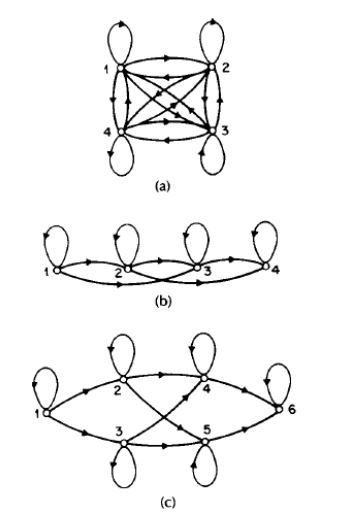
\includegraphics[width=10cm]{img/topohmm.jpg} % leia abaixo
\caption{Exemplo de topologias de HMM. a) Modelo ergódico b) Modelo esquerda-direita c) Modelo esquerda-direita paralelo. \textit{\cite{fundRecFala}}}
\label{fig:topohmm}
\end{figure}

\section{Os problemas a serem resolvidos}
\label{sec:3prob}
\quad O HMM possui três problemas básicos, que são:
\begin{enumerate}
\item \textbf{Problema de avaliação:} Dada a sequência de observação $O = (o_1, o_2, o_3, ..., o_n)$ e o modelo $\lambda = (A, B, \pi)$, como calcular eficientemente $P(o| \lambda)$.
\item \textbf{Problema da busca da melhor sequência de estados.}
\item \textbf{Problema de treinamento:} como ajustar os parâmetros do modelo $\lambda(A, B, \pi)$ para maximizar $P(o|\lambda)$.
\end{enumerate}

O problema 1, ou seja, o problema da avaliação pode ser solucionado através do procedimento \textit{Forward-Backward}. O segundo problema é solucionado com a aplicação do algoritmo de \textit{Viterbi} e o terceiro e último problema pode ser otimizado aplicando um procedimento iterativo como o método de \textit{Baum-Welch}. Nas seções \ref{secFB}, \ref{secViterbi} e \ref{secBW} faz-se uma explicação sobre os procedimentos para a solução dos problemas 1, 2 e 3 respectivamente.

\subsection{Foward-Backward}
\label{secFB}
Com a resolução do problema 1 podemos responder à algumas perguntas, se dado um modelo e uma sequência de observações, como podemos  saber de que a sequência observada foi produzido pelo modelo? ou, podemos ver essa  solução de outra forma,  um modelo é satisfatório para determinada entrada de observações?
 \begin{itemize}
\item Inicialização:\\
\begin{equation}
\displaystyle  \alpha_1 (i) = \pi_i b_i (O_1), \qquad 1 \leq i \leq N \\
\end{equation}

\item Indução:\\
$
\displaystyle \alpha_t + 1 (j) = \sum\limits_{ i = 1}^{N} \Big[\alpha_t(i) a_{ij} \Big]b_j (O_t + 1), \qquad 2 \leq t \leq T\\
%\displaystyle \Psi_t (j) = arg\max\limits_{1 \leq i \leq N}\Big[\delta_{t-1} (i)a_{ij}\Big], \qquad 1\leq j \leq N
$

\item Término:\\
$
P(O| \lambda) =  \sum\limits_{ i = 1}^{N} \Big[\alpha_t(i) \Big]\\
$

\end{itemize}

\subsection{Viterbi}
\label{secViterbi}
O algoritmo de Viterbi é um algoritmo de programação dinâmica usado para encontrar a sequência de estados ocultos ótima. Dado uma sequência de estados ocultos de um HMM, o algoritmo de viterbi calcula a melhor sequência de estados baseados nas probabilidades de transição. Este algoritmo foi proposto em 1967 por Andrew Viterbi para a decodificação de códigos convolucionais em links de comunicação ruidosos.  O algoritmo também possui aplicações  em redes CDMA e GSM, modem dial-up, satélites, síntese de fala, linguística computacional e bioinformática. Em telecomunicação, um código convolucional é um tipo de código corretor de erro em que cada conjunto de $m$ símbolos é transformado em um conjunto de $n$ símbolos.\\
Algoritmo
\begin{itemize}
\item Inicialização:\\
\begin{equation}
\delta_1 (i) = \pi_i b_i (O_1), \qquad 1 \leq i \leq N \\
\end{equation}
$
\quad \Psi_1 (i) = 0
$

\item Recursão:\\
\begin{equation}
\displaystyle \delta_t (j) = \max\limits_{1 \leq i \leq N} \Big[\delta_{t-1}(i) a_{ij} \Big]b_j (O_t), \qquad 2 \leq t \leq T\\
\end{equation}
\begin{equation}
\displaystyle \Psi_t (j) = arg\max\limits_{1 \leq i \leq N}\Big[\delta_{t-1} (i)a_{ij}\Big], \qquad 1\leq j \leq N
\end{equation}

\item Término:\\
\begin{equation}
\displaystyle P^* =\max\limits_{1 \leq i \leq N}  \Big[\delta_{T(i)}\Big] 
\end{equation}
\begin{equation}
\displaystyle G^*_T = arg\max\limits_{1 \leq i \leq N}  \Big[\delta_{T(i)}\Big]
\end{equation}


\end{itemize}





\subsection{Baum-Welch}
\label{secBW}
Não existe uma maneira conhecida de resolver analiticamente o conjunto de parâmetros para um dado modelo de forma que seja maximizada a probabilidade da seqüência de observações. No entanto um procediemento iterativo como o método de Baum-Welch  permite escolher $\lambda = (A, B, \pi)$ tal que $P(O|\lambda)$ é maximizada localmente. O algoritmo Baum-Welch é apresentado em termos das variáveis $\alpha_t$ e $\beta_t$ dos algoritmos forward e backward respectivamente, e segundo  \cite{artRabiner} é o mais indicado para a estimação dos parâmetros do HMM. A re-estimação dos parâmetros $a_{ij}$ e $b_{ij}$ para uma dada sequência de observações através do método de Baum-Welch é descrita da seguinte forma por [19].\\
Para uma única sequência de observações $O = {O_1, O_2, \ldots, O_T}$ a re-estimação da probabilidade de transição do estado $i$ para o estado $j$ da matriz de transição de estados $A$ é dada por:

$$
\displaystyle a_{ij} = \frac{\sum_{t=1}^{T-1} a_t(i)a_{ij}b_j (O_{t+1}) \beta_{t+1}(j)}{\sum_{t=1}^{T-1} a_t(i)\beta_t(j)}
$$

Para os HMM’s discretos, a quantidade de símbolos de saída é finita. Também para uma
única elocução, a re-estimação da função de probabilidade para que um estado $q_i$ emita um símbolo $O_t = V_k $ é obtida por:

$$
b_i(k) = \frac{\sum_{t=1}^{T-1} a_t(i)\beta_t(j) t.q. \quad O_t = V_k}{\sum_{t=1}^{T-1} a_t(i)\beta_t(j)}
$$

onde $ \displaystyle \qquad b_i(k) \geq 0, \qquad 1\leq i \leq N, \qquad 1 \leq k \leq M, \qquad \sum_{k=1}^M b_i(k) = 1, \qquad 1 \leq i \leq N$















\chapter{Resultados}
\thispagestyle{plain}
\quad Os métodos de estudados de filtragem de sinal, codificação de áudio e reconhecimento de fala foram implementados em linguagem computacional C, complilada  com GCC no sistema operacional Linux Ubuntu 12.04 LTS.

\section{Estrutura do Código}

\quad A estrtura das funções implementadas é mostrada na Figura \ref{fig:codigo}. 

\subsection{Captura e filtragem do sinal}

\quad A API utilizada para a captura de áudio foi a ALSA por meio de funções. Uma estrutura de programa básico usando esta API esta sempre na forma:

\begin{verbatim}
Abre uma interface para captura ou reprodução
setar os parâmetros de hardware
	Enquanto houver dados a serem processados:
		ler dados PCM
		ou escrever dados PCM
Fecha a interface
\end{verbatim}



%capitulo intitulado conclusao e obrigatorio
%\chapter{CONCLUS\~AO}
\label{chap:conclusao}
\thispagestyle{plain}
É a parte final do texto, na qual se apresentam conclusões correspondentes aos
objetivos ou hipóteses \cite[p.6]{NBR14724:2005}. Neste item podem também ser sugeridas ações
futuras a respeito do tema tratado.



% ---
% Finaliza a parte no bookmark do PDF, para que se inicie o bookmark na raiz
% ---
\bookmarksetup{startatroot}% 

% ----------------------------------------------------------
% ELEMENTOS PÓS-TEXTUAIS
% ----------------------------------------------------------
\postextual

% ----------------------------------------------------------
% Referências bibliográficas
% ----------------------------------------------------------
\bibliography{bib/tfg_referencias}


% ----------------------------------------------------------
% Glossário
% ----------------------------------------------------------
%\glossary
%
% ----------------------------------------------------------
% Apêndices e Anexos
% ----------------------------------------------------------
%\begin{apendicesenv}
% include(extra/00_apendice)
%\end{apendicesenv}
%\begin{anexosenv}
%\include{extra/01_anexo}
%\end{anexosenv}


%finaliza o documento 
\end{document}


